\documentclass{article}

\usepackage{Sweave}
\usepackage{slashbox}
\usepackage{subfig}
\begin{document}
\Sconcordance{concordance:PUTAPRUEBA.tex:PUTAPRUEBA.Rnw:%
1 135 1 1 2 1 0 4 1 7 0 1 2 10 1 1 2 1 0 4 1 7 0 1 2 90 1 1 2 1 0 1 3 2 %
0 3 1 7 0 1 2 2 1 1 2 1 0 3 1 7 0 1 2 58 1 1 2 1 0 5 1 4 0 1 2 1 1 1 2 %
1 0 1 1 9 0 1 3 1 1 1 2 1 0 1 1 6 0 1 2 12 1 1 2 1 0 5 1 4 0 1 2 1 1 1 %
2 1 0 1 1 6 0 1 2 1 1 1 2 1 0 1 1 6 0 1 2 300 1}

\Sconcordance{concordance:PUTAPRUEBA.tex:PUTAPRUEBA.Rnw:%
1 135 1 1 2 1 0 4 1 7 0 1 2 10 1 1 2 1 0 4 1 7 0 1 2 90 1 1 2 1 0 1 3 2 %
0 3 1 7 0 1 2 2 1 1 2 1 0 3 1 7 0 1 2 58 1 1 2 1 0 5 1 4 0 1 2 1 1 1 2 %
1 0 1 1 9 0 1 3 1 1 1 2 1 0 1 1 6 0 1 2 12 1 1 2 1 0 5 1 4 0 1 2 1 1 1 %
2 1 0 1 1 6 0 1 2 1 1 1 2 1 0 1 1 6 0 1 2 300 1}


\abstract{Tareas para entregar de la asignatura An\'alisis del Comportamiento Estrat\'egico. M\'aster en Econom\'ia.}
\section{Ejercicio 1:}

En el siguiente Juego a la Cournot la demanda de mercado que enfrentan n empresas es estrictamente convexa con la forma
$p(q)=\frac{a}{Q^\alpha}$, donde $Q=\sum_{i=1}^n q_i$. Los consumidores se asumen pasivos y vienen descritos por $p(Q)=a-bQ$.

\subsection{Empresas producen con $C_i(q_i)=cq_i$}
Si consideramos que el n\'umero de empresas \textbf{n} es 2, podemos calcular las cantidades que maximizan sus beneficios como:
 $$max\thinspace \pi_i(q_i)=q_i-cq_i$$
 condierando la maximizaci\'on de los beneficios de la empresa 1 tenemos:
 $$max\thinspace \pi_1(q_1)=(\frac{a}{(q_1+q_2)^\alpha})q_1-cq_1$$
podemos emplear derivadas parciales para obtener la condici\'on de primer orden:
  $$\frac{\partial(\pi_1(q_1,q_2)}{\partial q_1} = \frac{\partial}{\partial q_1} (\frac{aq_1}{cq_1+q_2)^\alpha})$$
  derivando podemos llegamos a la expresi\'on:
  $$-a\alpha q_1(q_1+q_2)^{-(\alpha+1)}+a(q_1+q_2)^{-\alpha}-c=0$$
  operando matematicamente podemos obtener $q_2=q_2(q_1)$:
$$q_2=\sqrt{\frac{\frac{-c}{a}}{\alpha q_1-1}}^{\frac{1}{\alpha-1}}$$
Esta funci\'on puede ser expresada en el espacio \{$q_1,q_2$\} como se aprecia en la siguiente figura:


\begin{Schunk}
\begin{Sinput}
> a=0.4; c=0.2; alfa=0.5
> q1=seq(0,0.999,by=0.01)
> q2=-q1+sqrt((-a/c)/(alfa*q1-1))
> plot(q1,q2)
\end{Sinput}
\end{Schunk}
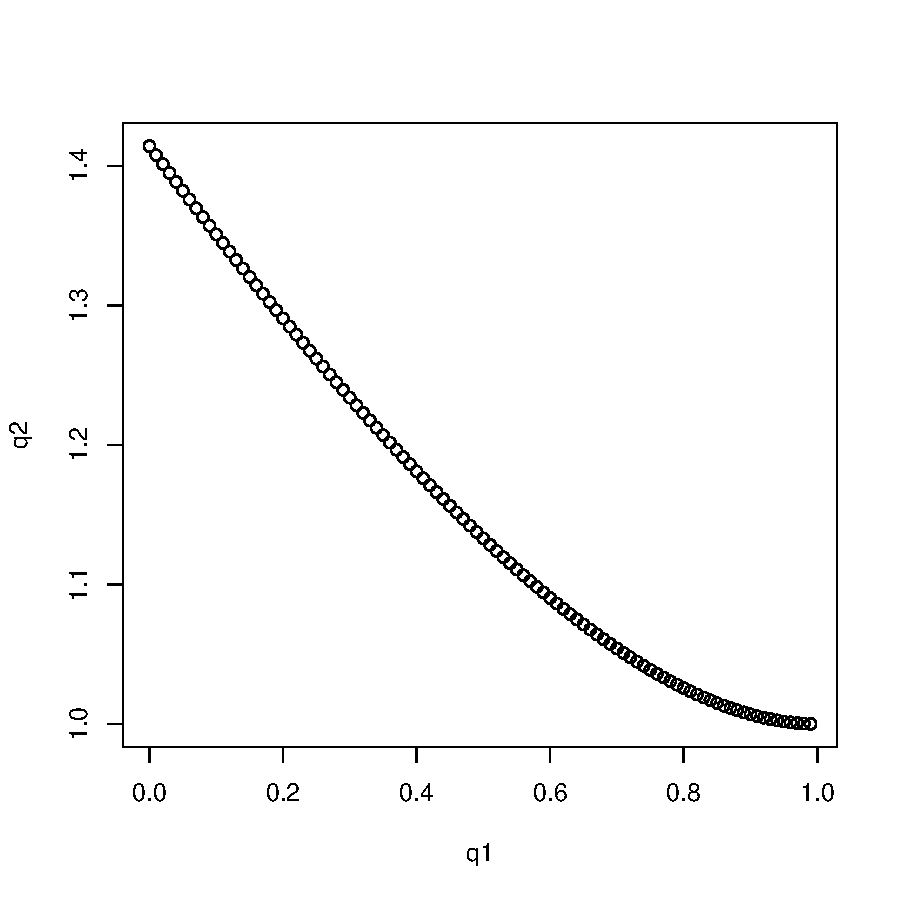
\includegraphics{PUTAPRUEBA-001}



Para resolver asignamos valores arbitrarios as variables (a>c). Vemos unha funci\'on decreciente. Ahora si sumonemos que las empresas producen un bien id\'entico $q_1=q_2$ podemos obterner una solución de la produci\'on con un programa de c\'alculo como R:

\begin{Schunk}
\begin{Sinput}
> p1=function(x){2*x-(sqrt((-a/c)/(alfa*x-1)))^(alfa-1)}
> plot(p1) 
> o1=uniroot(p1,c(0.1,1))
> (raiz1=o1$root)
\end{Sinput}
\begin{Soutput}
[1] 0.3977708
\end{Soutput}
\end{Schunk}
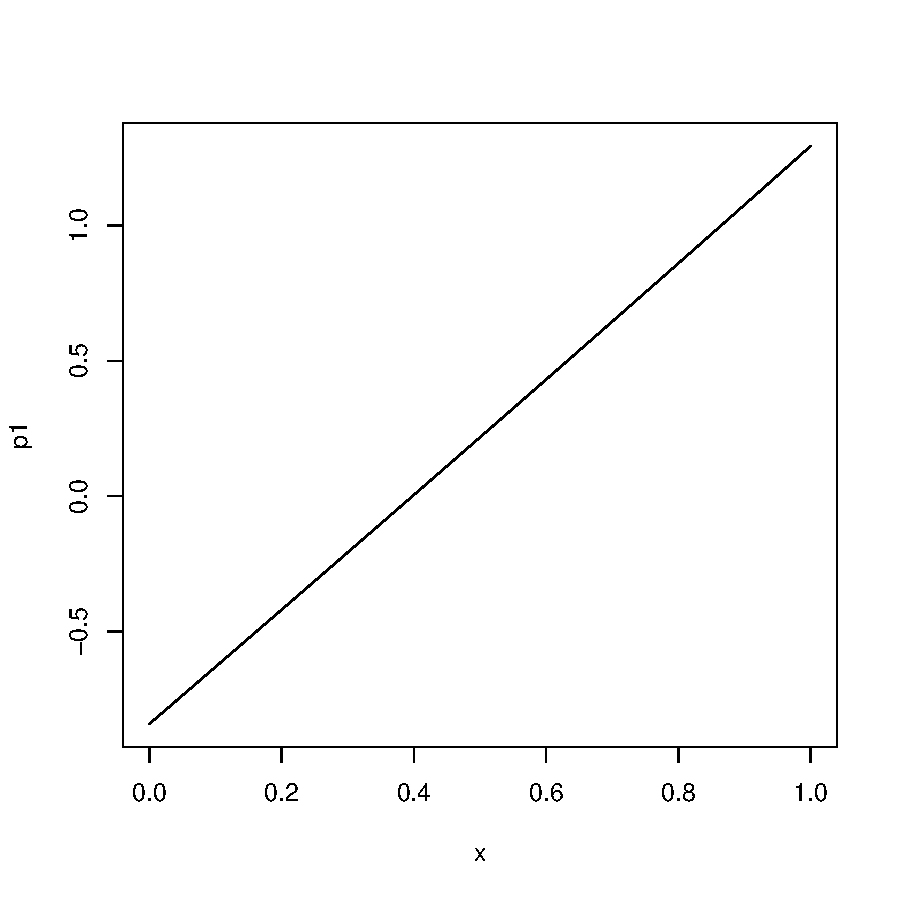
\includegraphics{PUTAPRUEBA-002}



Vemos que el programa nos arroja un valor de la produción de 0.399 cuando los bienes son homogeneos.

\subsection{Empresas producen con $C_i(q_i)=\frac{c}{2}q_i^2$}

\section{Ejercicio 2: Calcular ECN en condiciones generales}                     
\subsection{Para n empresas:}

$$Q=\sum_{i=1}^nq_i=q_i+\sum_{j\neq i}^nq_j$$             
$$p'(Q)<0; p''(Q)\geq0; p(Q)=a-Q$$                                
         
Las n empresas producen lo mismo: $Q=q_i+(n-1)q_{-i}$.
                                                                                                                                                                                              La funci\'on de beneficio para cada empresa i:            
$$\pi_i=p(Q)q_i-q_ic$$

Sustituyendo:
$$\pi_i=q_i(a-(q_i+(n-1)q_i)-c)=$$
$$q_i(a-q_i-(n-1)q_{-i}-c)=$$
$$aq_i-q_i^2-(n-1)q_{-i}q_i-cq_i$$

Derivando obtenemos la CPO:
$$\partial \pi_i/\partial q_i= a-2q_i-(n-1)q_{-i}-c=0$$

Extraemos la funci\'on de reacci\'on para cada i:
$$q_i=\frac{a-(n-1)q_{-i}-c}{2}$$

En equilibrio $q_i=q_{-i}$:
$$2q_i+(n-1)q_{-i}=a-c; (n+1)q_i=a-c;$$
$$q_i=\frac{a-c}{(n+1)}$$

$$Q=nq_i \rightarrow p=a-Q=a-n(\frac{a-c}{(n+1)}$$

Cuando el n\'umero de empresas tiende a infinito el precio tiende hacia el coste marginal:
$$\lim_{n\rightarrow \infty}a-n(\frac{a-c}{(n+1)}=a-a+c;$$
$$p=c$$

\subsection{Para 2 empresas:}

$$Q=q_i+q_j$$
$$p(Q)=a-Q; p(Q)=a-(q_i+q_j)$$

Definimos la funci\'on de beneficio para i y j:
$$\pi_i(q_i,q_j)=p(Q)q_i-cq_i=q_i(a-(q_i+q_j))-cq_i$$

Haciendo la derivada parcial obtenemos la CPO:
$$\partial \pi_i/\partial q_i= a-2q_i-q_j-c=0$$

As\'i, las mejores respuestas son:
$$q_i=\frac{a-c-q_j}{2}$$
$$q_j=\frac{a-c-q_j}{2}$$

Resolviendo:
$$q_i=q_j=\frac{(a-c)}{3}$$
$$p=a-Q=a-2(\frac{a-c}{3})=a-\frac{2}{3}a+\frac{2}{3}c=$$

ya que $a>c$:
$$\frac{1}{3}a+\frac{2}{3}c>c$$

Por lo tanto, el precio ser\'a mayor que el coste marginal generando beneficios extraordinarios para las empresas.

\section{Ejercicio 3:}
\section{Ejercicio 4:}

En este ejercicio intentaremos mostrar en juegos dinámicos de Cournot-Stackelberg mover primero no es siempre una ventaja. Vamos a emplear un mode similar al del Ejercicio 1, pero con costes crecientes de la forma $cq_i^3$.

\vspace{5mm}

Primero empezaremos por maximizar los beneficios de la empresa 2:

$$max\thinspace \pi_2(q_1,q_2)=aq_2-b(q_2+q_1)q_2-cq^3_2$$

obteniendo ahora la condici\'on de primer orden:

$$(\frac{\partial}{\partial q_1})(aq_2-b(q_2+q_1)q_2-cq^3_2)$$

obtenemos como soluci\'on:

$$q_2=\frac{2b+\sqrt{4b^2+12c(-q_1b+a)}}{6c}$$

esta es la cantidad de producci\'on que maximiza los beneficios de la empresa dos. Ahora maximizaremos los beneficios de la empresa uno considerando la produci\'on de la empresa dos que maximiza sus pripios beneficios $(q_2)$:

$$max\thinspace \pi_1(q_1,q_2)=aq_1-b(q_1+\frac{2b+\sqrt{4b^2+12c(-q_1b+a)}}{6c}q_1-cq^3_1$$

realizando la derivada parcial, con respecto a $q1$, y reordenando obtenemos la siguiente ecuación:

$$a-2bq_1+\frac{2b^2}{6c}+\frac{b}{6c}\frac{q_1(a+2b(9q_1+2))}{\sqrt{q_1^2(a+4(3bq_1+b)})}-3q_1^2=0$$

Para resolver esta ecuaci\'on anterior utilizaremos el siguiente Script de R:
\begin{Schunk}
\begin{Sinput}
> a=0.6 ;b=0.2 ;co=0.4 
> p1=function(x){a-2*b*x+2*b^2/(6*co)+(b/(6*co)*(x*(a+2*b*(9*x+2)))/
+ +                                        (sqrt((x^2)*(a+4*(3*b*x+b)))))-3*x^2}
> plot(p1) 
> o1=uniroot(p1,c(0.1,1))
> (raiz1=o1$root)
\end{Sinput}
\begin{Soutput}
[1] 0.4518852
\end{Soutput}
\end{Schunk}
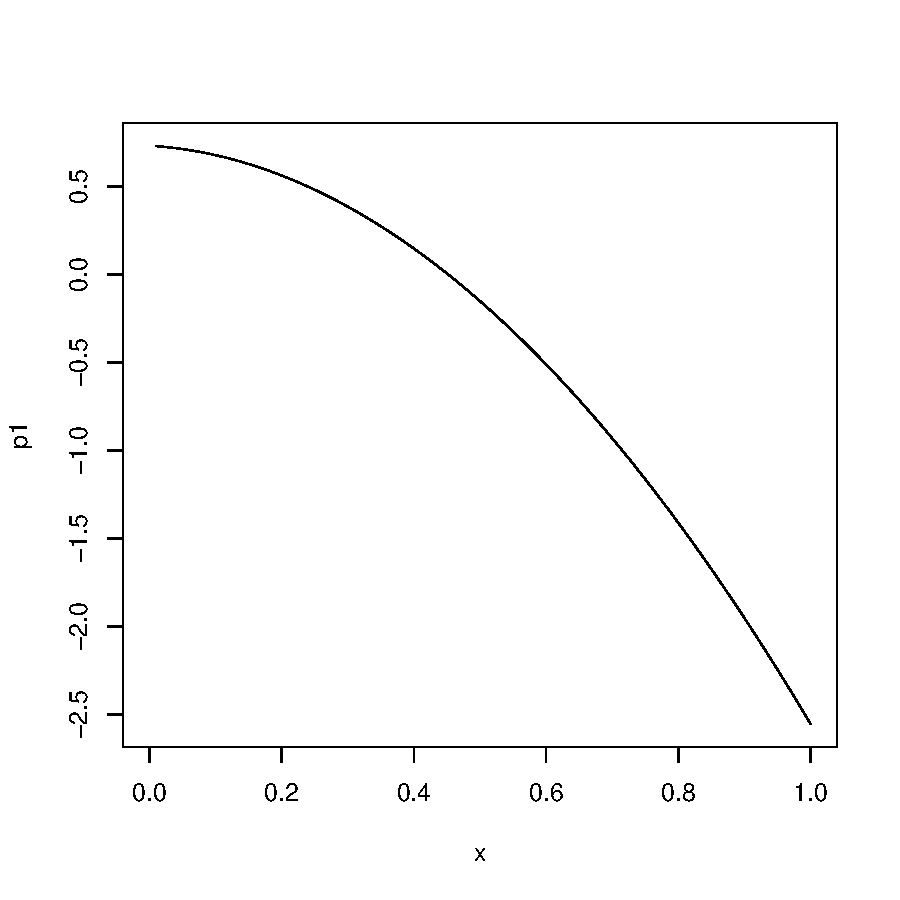
\includegraphics{PUTAPRUEBA-003}



\begin{Schunk}
\begin{Sinput}
> p2=function(x){6*co*x-2*b-sqrt(4*b^2+12*co*(-raiz1*b+a))}
> o2=uniroot(p2,c(0.1,1))
> plot(p2)
> (raiz2=o2$root)
\end{Sinput}
\begin{Soutput}
[1] 0.8393208
\end{Soutput}
\end{Schunk}
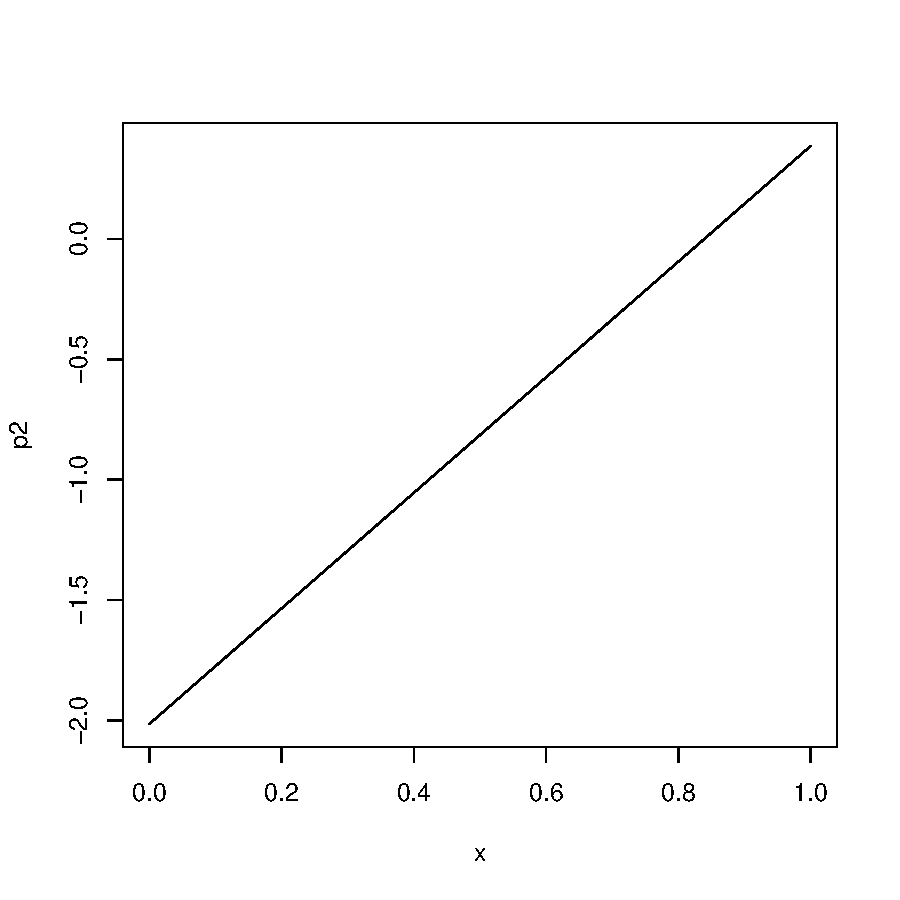
\includegraphics{PUTAPRUEBA-004}



Hemos dados valores aleatorios a las variables a, b y c y obtenemos la raiz de $q_1$. OS valores otorgados as variables son aleatorios pero teñen certa coherencia. a (m\'aima disposici\'on a pagar) es mayor que el coste marginal c. Por otro lado, como $b=0,2$ la pendiente de la demanda es muy pequeña por lo que la eslasticidade precio-demanda es muy grande.

Vemos de esta manera que la produci\'on de la empresa 1 ($q_1=0.45$) es inferior a la de la empresa 2 ($Q_2=0.83$) (supuesto que las empressas son homogeneass)



\section{Ejercicio 6:Generalizaci\'on de juego est\'atico con informaci\'on incompleta}
Consideremos las siguientes situaci\'on:
\begin{table}[htbp]
\begin{center}
\begin{tabular}{|l|l|l|l|}
\hline
1/2 & a & b & c \\
\hline \hline
A & 4,2 & 4,2 & 4,0 \\ \hline
B & 6,6 & 0,10 & 0,0 \\ \hline

\end{tabular}
\caption{Jugador 2 de tipo x}
\label{tabla:sencilla}
\end{center}
\end{table}

\begin{table}[htbp]
\begin{center}
\begin{tabular}{|l|l|l|l|}
\hline
1/2 & a & b & c \\
\hline \hline
A & 4,2 & 4,0 & 4,3 \\ \hline
B & 6,6 & 0,0 & 0,10 \\ \hline

\end{tabular}
\caption{Jugador 2 de tipo z}
\label{tabla:sencilla}
\end{center}
\end{table}



La probabilidad de que el jugador 2 sea de tipo x es p, as\'i mismo, la pobabilidad de que sea de tipo z es (1-p).


\subsection{Los dos jugadores tienen informaci\'on incompleta y sim\'etrica (por lo tanto ambos asignan las probabilidades p y (1-p))}

Al ser un juego simult\'aneo, el conjunto de estrategias coincide con el conjunto de acciones para cada jugador:
$$S_1=A_1=[A,B]$$
$$S_2=A_2=[a,b,c]$$

Supongamos, en primer lugar, que 1 juega A. Los valores esperados de jugar sus posibles acciones para el jugador 2 son:

$$VE^2_{(a)}=2p+(1-p)2=2$$
$$VE^2_{(b)}=2p+(1-p)0=2p$$
$$VE^2_{(c)}=0p+(1-p)3=1-3p$$

Programando estas funciones en R resulta f\'acil visualizar el VE para el jugador 2:
\begin{Schunk}
\begin{Sinput}
> a=function(p){2*p+(1-p)*2}
> b=function(p){2*p+(1-p)*0}
> d=function(p){p*0+(1-p)*3}
> plot(a, ylim=c(0,3.5))
> plot(b,add=TRUE)
> plot(d,add=TRUE)
\end{Sinput}
\end{Schunk}
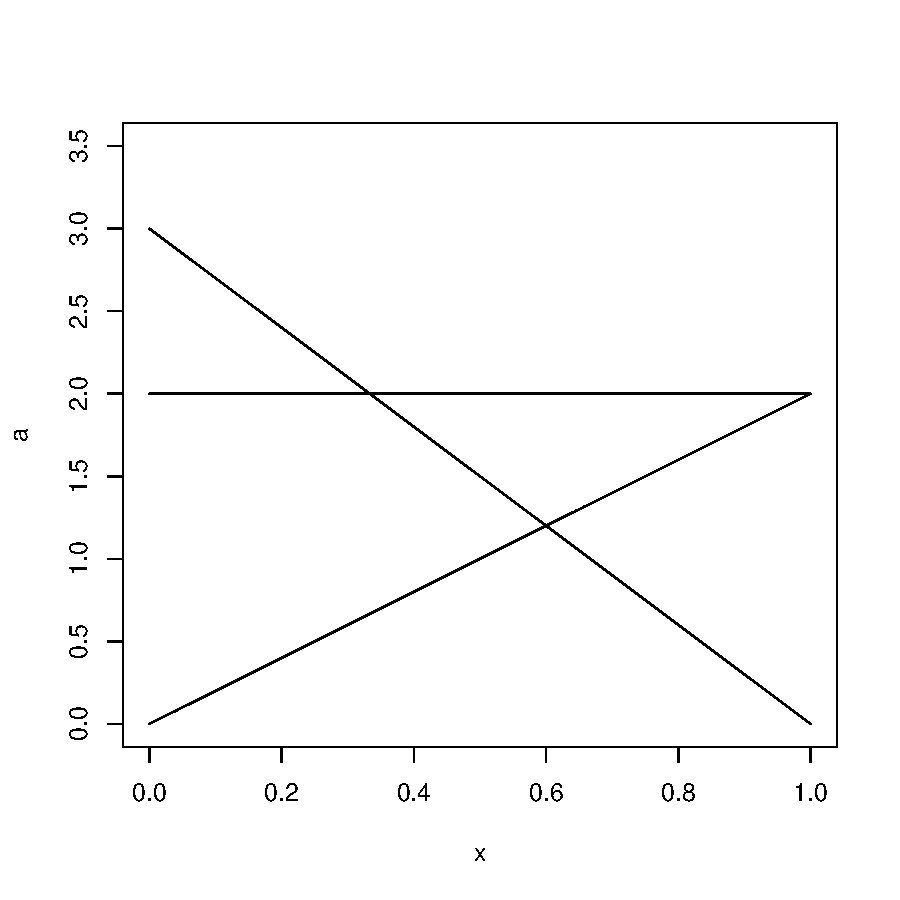
\includegraphics{PUTAPRUEBA-005}

Punto de corte entre d y a:
\begin{Schunk}
\begin{Sinput}
> t=function(p){(p*0+(1-p)*3)-2}
> (cortead=uniroot(t,c(0,1))$root) #punto de corte entre d y a
\end{Sinput}
\begin{Soutput}
[1] 0.3333333
\end{Soutput}
\begin{Sinput}
> 
\end{Sinput}
\end{Schunk}

Punto de corte entre a y c:
\begin{Schunk}
\begin{Sinput}
> g=function(p){(2*p+(1-p)*2)-(2*p+(1-p)*0)}
> (corteab=uniroot(g,c(0,1))$root)
\end{Sinput}
\begin{Soutput}
[1] 1
\end{Soutput}
\end{Schunk}

Dando lugar a la siguiente funci\'on de reacci\'on para el jugador 2:

$$\left\{ \begin{array}{c} b, si p<1/3\\ a, si 1/3<p<1\\b,a, si: p=1\end{array}\right. $$


Si 1 juega B:
$$VE^2_{(a)}=6p+(1-p)6=6$$
$$VE^2_{(b)}=10p+(1-p)0=10p$$
$$VE^2_{(c)}=0p+(1-p)10=1-10p$$

Graficando el VE para el jugador 2:

\begin{Schunk}
\begin{Sinput}
> a=function(p){6*p+(1-p)*6}
> b=function(p){10*p+(1-p)*0}
> d=function(p){p*0+(1-p)*10}
> plot(a, ylim=c(0,10))
> plot(b,add=TRUE)
> plot(d,add=TRUE)
\end{Sinput}
\end{Schunk}
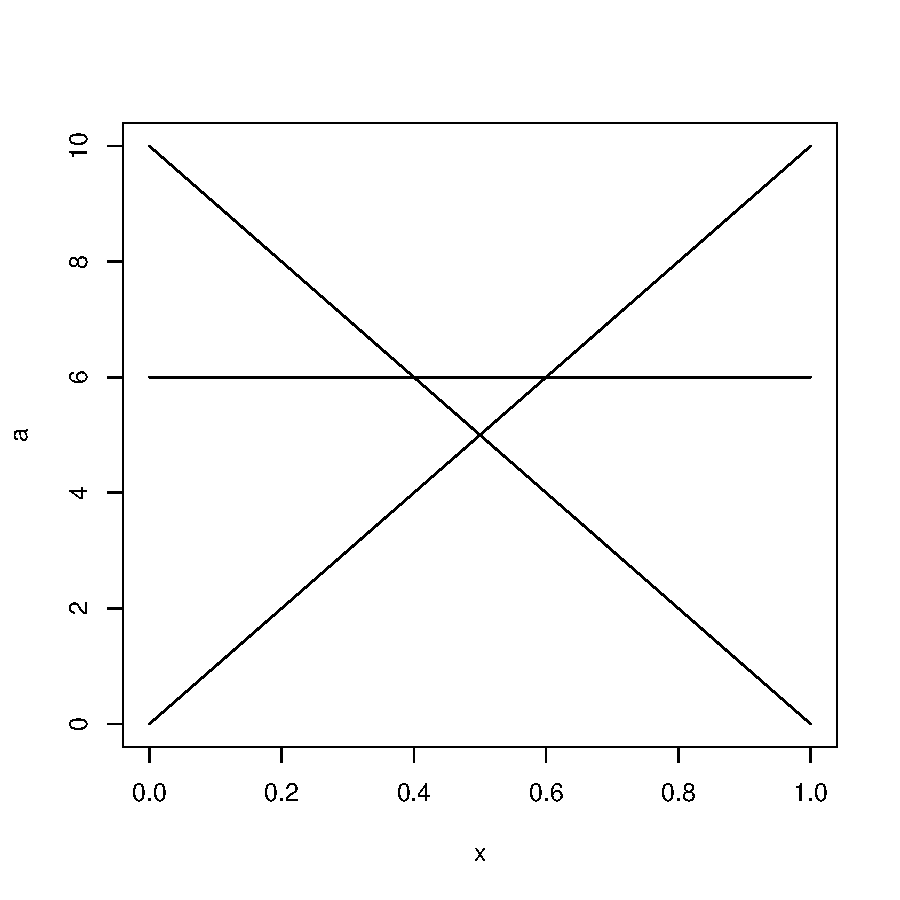
\includegraphics{PUTAPRUEBA-008}

Puntos de corte:
\begin{Schunk}
\begin{Sinput}
> k=function(p){(p*0+(1-p)*10)-(6*p+(1-p)*6)}
> (corte1=uniroot(k,c(0,1))$root)
\end{Sinput}
\begin{Soutput}
[1] 0.4
\end{Soutput}
\end{Schunk}

Y:
\begin{Schunk}
\begin{Sinput}
> m=function(p){(10*p+(1-p)*0)-(6*p+(1-p)*6)}
> (corte2=uniroot(m,c(0,1))$root)
\end{Sinput}
\begin{Soutput}
[1] 0.6
\end{Soutput}
\end{Schunk}

Obtenemos la funci\'on de reacci\'on para el jugador 2 cuando el jugador 1 juega B:

$$\left\{ \begin{array}{c} b, si p<0.4 \\ a, si 0.4<p<0.6\\c, si: p>0.6\end{array}\right. $$

As\'i, podemos obtener los Equilibrios de Nash correspondientes a todo el espectro de posibles probabilidades subjetivas p y (1-p):

Para p<1/3; El jugador 2 juega:
  c si 1 juega A
  b si 1 juega B
  
Puesto que en esta situaci???n A es una estrategia dominante para el jugador 1, el Equilibrio de Nash ser\'ia (c,A).

Para 1/3<p<0.4; Existen 2 equilibrios de Nash: (a,A) y (b,B).

Para 0.4<p<0.6; El jugador 2 juega siempre a y el jugador 1 B; Equilibrio de Nash: (a,B).

Para p>0.6; Equilibrio de Nash: (a,A), (c,B).


\subsection{solo el jugador 1 desconoce el tipo del jugador 2}

Si 2 es de tipo x, mejor respuesta de 2:
$$MR^2_{(A)}=a,b$$
$$MR^2_{(B)}=b$$

Mejor respuesta de 1:
$$MR^1_{(a)}=B$$
$$MR^1_{(b)}=A$$
$$MR^1_{(c)}=A$$

As\'i, el Equilibrio de Nash si 2 es de tipo x es (b,A)


Si 2 es de tipo z, mejor respuesta de 2:
$$MR^2_{(A)}=c$$
$$MR^2_{(B)}=c$$

Mejor respuesta de 1:
$$MR^1_{(a)}=B$$
$$MR^1_{(b)}=A$$
$$MR^1_{(c)}=A$$

As\'i, el Equilibrio de Nash si 2 es de tipo z es (C,A)

\section{Ejercicio 7: Competencia Bertrand con informaci\'on incompleta}

Competencia Bertrand con producto homog\'eneo, es decir, $d=1$:

El coste marginal de la empresa 1 puede ser $\bar{c}$ o $\underline{c}$.
El coste marginal de la empresa 2 es c con certeza.
Se cumple:
$$0<\underline{c}<c<\bar{c}$$

La empresa 2 conoce la distribuci\'on de probabilidad del coste marginal de la empresa 1, es decir, sabe que el coste la empresa 1 es $\underline{c}$ con probabilidad $\gamma$; $0<\gamma<1$ y $\bar{c}$ con probabilidad $(1-\gamma)$.

La funci\'on de demanda residual de la empresa es $q_i(p_i,p_j)=a-p_i+dp_j$. Sabiendo que $d=1$ para productos homog\'eneos (m\'aximo grado de substituci\'on) obtenemos:
$$q_i(p_i,p_j)=a-p_i+p_j$$ $$i,j=1,2$$ $$i\neq j$$

La estrategia \'optima para cada empresa es decidir el precio que constituya la mejor respuesta apra cada uno de los tipos  en los que podr\'ia encarnarse. As\'i, sus mejores respuestas provendr\'an de la maximizaci\'on de sus funciones de beneficios.

Para 1 si su tipo es $\underline{c}$:
$$\pi_1(p_1,p_2)=(p_1-\underline{c})(a-p_1+p_2)$$

CPO:
$$p_1(\underline{c};p_2)=\frac{a+\underline{c}+dp_2}{2}$$

Para 1 si su tipo es $\bar{c}$:
$$\pi_1(p_1,p_2)=(p_1-\bar{c})(a-p_1+p_2)$$

CPO:
$$p_1(\bar{c};p_2)=\frac{a+\bar{c}+dp_2}{2}$$

Para la empresa 2, la funci\'on de beneficios esperados ser\'a:
$$E[\pi_2]=(p_2-c)[\gamma(a-p_2+p_1(\underline{c})+(1-\gamma)(a-p_2+p_1(\bar{c}))]$$

El precio \'optimo que fijar\'a la empresa 2 de acuerdo con sus creencias sobre los costes de la empresa 1 ser\'a:
$$p_2(c;p_1(\underline{c}),p_1(\bar{c}))=\frac{a+c+(\gamma p_1(\underline{c})+(1-\gamma)p_1(\bar{c}))}{2}$$

Resolviendo, el EB de el duopolio con bien homog\'eneo e informaci\'on incompleta de Bertrand es el perfil de estrategias:

$${(p_1^*(\underline{c}),p_1^*(\bar{c}),p_2^*)}={(\frac{6a-(4-(1+\gamma))\underline{c}+(1-\gamma)\bar{c}+c}{6},\frac{6a+(4-\gamma)\bar{c}+\gamma \underline{c}+2c}{6},\frac{3a+2c+(\gamma \underline{c}+(1-\gamma)\bar{c})}{3})}$$




\section{Ejercicio 8:Subastas}
\subsection{Sobre cerrado segundo precio.}
Investigar qu\'e sueder\'ia con la estrategia $b_i^`(v_i)<v_i$, es decir, cuando el jugador puja una cantidad de dinero superior a su valoraci\'on.

Se pueden presentar los siguientes casos:

1.-Gana la subasta si $b'_i(v_i)>\bar{b}$, obteniendo un pago de $v_i-b'_i(v_i)<0$.

2.-Gana la subasta si $b'_i(v_i)>\bar{b}$, pero obtiene un pago negativo de $v_i-b'_i(v_i)<0$. Esto sucede cuando $b'_i(v_i)-\bar{b}$ > $v_i-\bar{b}$.

3.-Pierde la subasta si $b'_i(v_i)<\bar{b}$.

\subsection{Sobre cerrado al primer precio}

En este tipo de subastas, el ganador es aquel jugador que ofreciese la puja m\'as alta. El pago ser\'a su ropia oferta. Adem\'as, los jugadores no pueden ver las pujas de los dem\'as.

Calcular la MRi y obtener EBN.

Conjunto de acciones posibles para cada jugador: $i=1,..,n$. Se corresponde con el conjunto de pujas que puede ofertar.
El conjunto de acciones y de estrategias coincide al ser un juego simult\'aneo:
$$A_i=S_i=[0,+\infty)$$

Los tipos de cada jugador i son las distintas valoraciones que puede tener del objeto subastado:
$$T_i=[0,\bar{v}]$$

Cada i cree que el resto de valoraciones $v_j$ est\'a uniformemente distribuida en $[0,\bar{v}]$.

El pago de cada jugador es su beneficio esperado.

El objetivo de cada jugador es maximizar el beneficio.

En esta situaci\'on, el EB ser\'a el perfil de pujas:
$${(b_1^*,...,b_n^*)}={(\frac{n-1}{n}v_1,...,\frac{n-1}{n}v_n)}$$

No hay estrategia dominante, cada jugador debe determinar su mejor respuesta frente a la estrategia de los dem\'as.

Definimos la probabilidad de que i puje por debajo de b:
$$Pr(B_i\leq b)=Pr(v_i\leq B^{-1}(b))=F(B^{-1}(b))=\frac{B^{-1(b)}}{\bar{v}}$$

Todo jugador distinto de i puede saber con qu\'probabilidad ganar\'a la subasta conociendo la probabilidad anterior, esto se debe a que cuando puja b, conoce la probabilidad de que i puje menos que b.

La probabilidad de que todos los jugadores menos el jugador 1 pujen menos que b es:
$$Pr(B_i\leq b, \forall i=2,3,...,n)=(\frac{B^{-1(b)}}{\bar{v}})^{n-1}$$
 Por lo tanto, esta es la probabilidad de que 1 gane la subasta puando b.

La utilidad esperada de 1 pujando b es:
$$E[u_1]=(v_1-b)(\frac{B^{-1(b)}}{\bar{v}})^{n-1}$$

Teniedo en cuenta que si gana obtiene $v_1-b$, y si pierde obtiene 0.

Maximizando la utilidad esperada obtenemos la siguiente CPO:
$$\partial E[u_1]/\partial b=0=(-1)(\frac{B^{-1(b)}}{\bar{v}})^{n-1}+(v_1-b)(n-1)(\frac{B^{-1(b)}}{\bar{v}})^{n-2}\frac{1}{\bar{v}}\frac{dB^{-1}(b)}{db}$$

Reescribiendo:
$$(\frac{B^{-1(b)}}{\bar{v}})^{n-1}=(v_1-b)(n-1)(\frac{B^{-1(b)}}{\bar{v}})^{n-2}\frac{1}{\bar{v}}\frac{dB^{-1}(b)}{db}$$

Simplificando:
$$B^{-1}(b)\frac{dB}{dv}(B^{-1}(b))=(v_1-b)(n-1)$$

Asumiendo todos los jugadores sim\'etricos: $B^{-1}(b)=v_1$ y $b=B(v_1)$; As\'i:
$$\frac{dB}{dv}(v)=(1-\frac{B(v)}{v})(n-1)$$

Esta expresi\'on es una ecuaci\'on diferencial ordinaria de primer orden. Fijando la condici\'on $B(0)=0$ (La puja de un jugador con valoraci\'on nula es igual a 0) se obtiene:
$$B(v)=\frac{n-1}{n}v$$

Esta expresi\'on denota la relaci\'on existente entre la puja de cada jugador y su valoraci\'on. Como $\frac{n-1}{n}<1$, los jugadores pujan por debajo de sus verdaderas valoraciones en el EB.



\section{Ejercicio 9:Provisi\'on de bien p\'ublico}
\subsection{Modificaci\'on de pagos para que ninguno de los dos agentes tenga estrategia dominante.}
En este ejercicio en un caso de provisión de un bien p\'ublico consideramos: Una familia formada por los individuos 1 y 2 los cuales deben decidir simultaneamente y puede decidir contribuir o no contribuir, $\{C,N\}_i, i=1,2$. El bien p\'ublico se suministrar\'a si alguno de los individuos o \'ambos eligen contribuir. Contribuir a financiar el bien p\'ublio le supone al jugador 1 un coste de $c_1$ y al individuo 2 un coste que puede ser $\overline{c_2}$ o $\underline{c_2}$. El individuo 2 los costes que le supone al individuo 1 pero este \'ultimo no conoce los costes para le individuo 2(lo único que sabe es que ouede ser $\overline{c_2}$ con probabilidad $\frac{1}{3}$ o $\underline{c_2}$ con probabilidad $\frac{2}{3}$).

\hspace{2cm}

La tarea propuesta es considerando el caso de los apuntes, modificar los pagos (los cuales mostraremos tabulados) para que el individuo 2 no posea una estrategia dominante como es la de contribuir. Para eso modificamos los pagos de la forma:

\hspace{2cm}

\begin{table}[tbp]
\centering
\begin{minipage}[b]{0.5\linewidth}
\begin{tabular}{|l|r|r|}
\hline
\backslashbox{1}{2} & C & N \\
\hline
C & $1-c_1,1-\underline{c_2}$ & 1-$c-1$,1\\
\hline
N & 1,1-$\overline{c_2}$ & 0,2\\
\hline
\end{tabular}
\caption{Jugador 2 del tipo $\overline{c_2}$ }
\end{minipage}

\hspace{0.5cm} 

\begin{minipage}[b]{0.5\linewidth}
\begin{tabular}{|l|r|r|}
\hline
\backslashbox{1}{2} & C & N \\
\hline
C & 1-$c_1$,1-$\underline{c_2}$ & 1-$c_1$,1\\
\hline
N & 1,1-$\underline{c_2}$ & 0,0\\
\hline
\end{tabular}
\caption{Jugador 2 del tipo $\underline{c_2}$}
\end{minipage}
\end{table}

El principal cambio realizado es el pago de 2 cuando es de tipo $\overline{c_2}$ y 1 elige no contribuir. Con este cambio el individuo 2 cunando es de tipo $\overline{c_2}$ tendr\'a la estrategia dominante de no contribuir.
Con estes pagos si analizamos los valores esperados con la finalidad de obtener la mejor respuestas del individuo 2 vemos que:

\hspace{0.5cm} 

Si el individuo 2 es de tipo $\overline{c_2}$:

$$E(u_2,\overline{c_2},1C)\Longrightarrow (1-c \overline{c_2})\gamma+(1-\gamma)$$
$$E(u_2,\overline{c_2},1N)\Longrightarrow (1-c \overline{c_2})\gamma+2(1-\gamma)$$

Si el individuo 2 es de tipo $\underline{c_2}$:

$$E(u_2,\underline{c_2},1C)\Longrightarrow (1-c \underline{c_2})\gamma+(\gamma-1)$$
$$E(u_2,\underline{c_2},1N)\Longrightarrow (1-c \underline{c_2})\gamma+0$$

Vemos con esto los valores esperados el individuo 2 tendr\'a una estrategia dominante dependiente de su tipo.

Ahora analizaremos los pagos esperados del individuo 1, que asigna una probabilidad $\mu$ a que le individuo 2 sea de tipo $\bar{c_2}$ y elija N y una probabbilidad $\lambda$ a que el ndividuo 2 sea de tipo $\underline{c_2}$ y elija C.

Si el individuo 1 elige C 

$$E(u_1,C)=\frac{2}{3}(1-\mu)(1-c_1)+\frac{1}{3}\lambda(1-c_1)+\frac{2}{3}(1-c_1)+\frac{1}{3}(1-\lambda)(1-c_1)=1-c_1$$

Si el individuo q elije N

$$E(u_1,N)=\frac{2}{3}(1-\mu)(1-c_1)+\frac{1}{3}\lambda$$

Las mejores respestas del individuo 1 son:

$$\left\{ \begin{array}{c} C si c_1<\frac{1}{3}(2\mu-\lambda+1) \\ N si c_1>\frac{1}{3}(2\mu-\lambda+1)\end{array}\right. $$


Por lo tanto tenemos que si $c$ es suficientemente bajo

-Si el individuo 1 toma la estrategia  i$S_1^*=C$ el individuo 2 tiene las estrategias $S_2^*(\underline{c_2}=C$ $$S_2^*(\overline{c_2}=N$$. Si $S_1^*=N$ 

-Si el individuo 1 toma la estrategia  i$S_1^*=N$ el individuo 2 tiene las estrategias $S_2^*(\underline{c_2}=C$ $$S_2^*(\overline{c_2}=N$$. Si $S_1^*=N$ 


Y si $c$ es suficientemente grande y el individuo 2 es de tipo $\overline{c_2}$ ninguno de los individuos optar\'a por contribuir.



\subsection{Generalizar el modelo con el sistema de creencias $(p,1-p)$.}










\end{document}
